\documentclass[12pt]{article}
\usepackage[left=1cm, right=1cm, top=2cm,bottom=1.5cm]{geometry} 

\usepackage[parfill]{parskip}
\usepackage[utf8]{inputenc}
\usepackage[T2A]{fontenc}
\usepackage[russian]{babel}
\usepackage{enumitem}
\usepackage[normalem]{ulem}
\usepackage{amsfonts, amsmath, amsthm, amssymb, mathtools,xcolor,accents}
\usepackage{blkarray}

\usepackage{tabularx}
\usepackage{hhline}

\usepackage{accents}
\usepackage{fancyhdr}
\pagestyle{fancy}
\renewcommand{\headrulewidth}{1.5pt}
\renewcommand{\footrulewidth}{1pt}

\usepackage{graphicx}
\usepackage[figurename=Рис.]{caption}
\usepackage{subcaption}
\usepackage{float}

%%Наименование папки откуда забирать изображения
\graphicspath{ {./images/} }

%%Изменение формата для ввода доказательства
\renewcommand{\proofname}{$\square$  \nopunct}
\renewcommand\qedsymbol{$\blacksquare$}

%%Изменение отступа на таблицах
\addto\captionsrussian{%
	\renewcommand{\proofname}{$\square$ \nopunct}%
}
%% Римские цифры
\newcommand{\RN}[1]{%
	\textup{\uppercase\expandafter{\romannumeral#1}}%
}

%% Для удобства записи
\newcommand{\MR}{\mathbb{R}}
\newcommand{\MC}{\mathbb{C}}
\newcommand{\MQ}{\mathbb{Q}}
\newcommand{\MN}{\mathbb{N}}
\newcommand{\MZ}{\mathbb{Z}}
\newcommand{\MTB}{\mathbb{T}}
\newcommand{\MTI}{\mathbb{I}}
\newcommand{\MI}{\mathrm{I}}
\newcommand{\MCI}{\mathcal{I}}
\newcommand{\MJ}{\mathrm{J}}
\newcommand{\MH}{\mathrm{H}}
\newcommand{\MT}{\mathrm{T}}
\newcommand{\MU}{\mathcal{U}}
\newcommand{\MV}{\mathcal{V}}
\newcommand{\MB}{\mathcal{B}}
\newcommand{\MF}{\mathcal{F}}
\newcommand{\MW}{\mathcal{W}}
\newcommand{\ML}{\mathcal{L}}
\newcommand{\MP}{\mathcal{P}}
\newcommand{\VN}{\varnothing}
\newcommand{\VE}{\varepsilon}
\newcommand{\dx}{\, dx}
\newcommand{\dy}{\, dy}
\newcommand{\dz}{\, dz}
\newcommand{\dd}{\, d}


\theoremstyle{definition}
\newtheorem{defn}{Опр:}
\newtheorem{rem}{Rm:}
\newtheorem{prop}{Утв.}
\newtheorem{exrc}{Упр.}
\newtheorem{problem}{Задача}
\newtheorem{lemma}{Лемма}
\newtheorem{theorem}{Теорема}
\newtheorem{corollary}{Следствие}

\newenvironment{cusdefn}[1]
{\renewcommand\thedefn{#1}\defn}
{\enddefn}

\DeclareRobustCommand{\divby}{%
	\mathrel{\text{\vbox{\baselineskip.65ex\lineskiplimit0pt\hbox{.}\hbox{.}\hbox{.}}}}%
}
\DeclareRobustCommand{\ndivby}{\mkern-1mu\not\mathrel{\mkern4.5mu\divby}\mkern1mu}


%Короткий минус
\DeclareMathSymbol{\SMN}{\mathbin}{AMSa}{"39}
%Длинная шапка
\newcommand{\overbar}[1]{\mkern 1.5mu\overline{\mkern-1.5mu#1\mkern-1.5mu}\mkern 1.5mu}
%Функция знака
\DeclareMathOperator{\sgn}{sgn}

%Функция ранга
\DeclareMathOperator{\rk}{\text{rk}}
\DeclareMathOperator{\diam}{\text{diam}}


%Обозначение константы
\DeclareMathOperator{\const}{\text{const}}

\DeclareMathOperator{\codim}{\text{codim}}

\DeclareMathOperator*{\dsum}{\displaystyle\sum}
\newcommand{\ddsum}[2]{\displaystyle\sum\limits_{#1}^{#2}}
\newcommand{\ddssum}[2]{\displaystyle\smashoperator{\sum\limits_{#1}^{#2}}}
\newcommand{\ddlsum}[2]{\displaystyle\smashoperator[l]{\sum\limits_{#1}^{#2}}}
\newcommand{\ddrsum}[2]{\displaystyle\smashoperator[r]{\sum\limits_{#1}^{#2}}}

%Интеграл в большом формате
\DeclareMathOperator{\dint}{\displaystyle\int}
\newcommand{\ddint}[2]{\displaystyle\int\limits_{#1}^{#2}}
\newcommand{\ssum}[1]{\displaystyle \sum\limits_{n=1}^{\infty}{#1}_n}

\newcommand{\smallerrel}[1]{\mathrel{\mathpalette\smallerrelaux{#1}}}
\newcommand{\smallerrelaux}[2]{\raisebox{.1ex}{\scalebox{.75}{$#1#2$}}}

\newcommand{\smallin}{\smallerrel{\in}}
\newcommand{\smallnotin}{\smallerrel{\notin}}

\newcommand*{\medcap}{\mathbin{\scalebox{1.25}{\ensuremath{\cap}}}}%
\newcommand*{\medcup}{\mathbin{\scalebox{1.25}{\ensuremath{\cup}}}}%

\makeatletter
\newcommand{\vast}{\bBigg@{3.5}}
\newcommand{\Vast}{\bBigg@{5}}
\makeatother

%Промежуточное значение для sup\inf, поскольку они имеют разную высоту
\newcommand{\newsup}{\mathop{\smash{\mathrm{sup}}}}
\newcommand{\newinf}{\mathop{\mathrm{inf}\vphantom{\mathrm{sup}}}}

%Скалярное произведение
\newcommand{\inner}[2]{\left\langle #1, #2 \right\rangle }
\newcommand{\linsp}[1]{\left\langle #1 \right\rangle }
\newcommand{\linmer}[2]{\left\langle #1 \vert #2\right\rangle }

%Подпись символов снизу
\newcommand{\ubar}[1]{\underaccent{\bar}{#1}}

%%Шапка для букв сверху
\newcommand{\wte}[1]{\widetilde{#1}}
\newcommand{\wht}[1]{\widehat{#1}}
\newcommand{\ovl}[1]{\overline{#1}}


%%Трансформация Фурье
\newcommand{\fourt}[1]{\mathcal{F}\left(#1\right)}
\newcommand{\ifourt}[1]{\mathcal{F}^{-1}\left(#1\right)}

%%Символ вектора
\newcommand{\vecm}[1]{\overrightarrow{#1\,}}

%%Пространстов матриц
\newcommand{\matsq}[1]{\operatorname{Mat}_{#1}}
\newcommand{\mat}[2]{\operatorname{Mat}_{#1, #2}}

%Оператор для действ и мнимых чисел
\DeclareMathOperator{\IM}{\operatorname{Im}}
\DeclareMathOperator{\RE}{\operatorname{Re}}
\DeclareMathOperator{\li}{\operatorname{li}}
\DeclareMathOperator{\GL}{\operatorname{GL}}
\DeclareMathOperator{\SL}{\operatorname{SL}}
\DeclareMathOperator{\Char}{\operatorname{char}}
\DeclareMathOperator\Arg{Arg}
\DeclareMathOperator\ord{ord}

%Оператор для образа
\DeclareMathOperator{\Ima}{Im}

%Делимость чисел
\newcommand{\modn}[3]{#1 \equiv #2 \; (\bmod \; #3)}
\newcommand{\nmodn}[3]{#1 \not\equiv #2 \; (\bmod \; #3)}

%%Взятие в скобки, модули и норму
\newcommand{\parfit}[1]{\left( #1 \right)}
\newcommand{\modfit}[1]{\left| #1 \right|}
\newcommand{\sqparfit}[1]{\left\{ #1 \right\}}
\newcommand{\normfit}[1]{\left\| #1 \right\|}

%%Функция для обозначения равномерной сходимости по множеству
\newcommand{\uconv}[1]{\overset{#1}{\rightrightarrows}}
\newcommand{\uconvm}[2]{\overset{#1}{\underset{#2}{\rightrightarrows}}}

%% Функция для добавления круга сверху множества
\newcommand{\Circ}[1]{\accentset{\circ}{#1}}

%%Функция для обозначения нижнего и верхнего интегралов
\def\upint{\mathchoice%
	{\mkern13mu\overline{\vphantom{\intop}\mkern7mu}\mkern-20mu}%
	{\mkern7mu\overline{\vphantom{\intop}\mkern7mu}\mkern-14mu}%
	{\mkern7mu\overline{\vphantom{\intop}\mkern7mu}\mkern-14mu}%
	{\mkern7mu\overline{\vphantom{\intop}\mkern7mu}\mkern-14mu}%
	\int}
\def\lowint{\mkern3mu\underline{\vphantom{\intop}\mkern7mu}\mkern-10mu\int}

%%След матрицы
\DeclareMathOperator*{\tr}{tr}

\makeatletter
\renewcommand*\env@matrix[1][*\c@MaxMatrixCols c]{%
	\hskip -\arraycolsep
	\let\@ifnextchar\new@ifnextchar
	\array{#1}}
\makeatother


%% Переопределение функции хи, чтобы выглядела более приятно
\makeatletter
\@ifdefinable\@latex@chi{\let\@latex@chi\chi}
\renewcommand*\chi{{\@latex@chi\smash[t]{\mathstrut}}} % want only bottom half of \mathstrut
\makeatletter

\setcounter{MaxMatrixCols}{20}

\begin{document}
\lhead{Математический анализ - \RN{4}}
\chead{Шапошников С.В.}
\rhead{Лекция - 6}
\section*{Формула замены переменных}
\begin{prop}
	Пусть $\MU$ - открытое множество в $\MR^n$, тогда $\MU$ - это объединение не более, чем счётного набора замкнутых кубов, которые пересекаются лишь по границе:
	$$
		\MU = \bigcup\limits_{m}K_m, \, K_m \text{ - замкнутый куб}, \, \forall i,j, \, K_i \cap K_j \subset \partial K_i \cup \partial K_j
	$$
\end{prop}
\begin{prop}
	В определении множества меры нуль по Лебегу произвольные бруски можно заменить кубами.
\end{prop}

\begin{prop}
	Пусть $\MU$ - открытое множество $\subset \MR^n$, $f\colon \MU \to \MR^k, \, k \geq n$ - локально Липшицева, то есть 
	$$
		\forall\,  \MI \text{ - замкнутый брус } \subset \MU, \, \exists \, L > 0 \colon \forall x,y \in \MI, \, \|f(x) - f(y)\| \leq L{\cdot}\|x -y \|
	$$
	Тогда для всякого множества $E \subset \MU$ меры нуль множество $f(E)$ является множеством меры нуль.
\end{prop}
\begin{proof}
	Возьмем множество $E \subset \MU$ - множество меры нуль по Лебегу. Мы знаем, что $\MU = \cup_m K_m$ - счетное объединение кубов. Тогда множество $E$ можно представить, как: $E = \cup_m E_m$, где $\forall m, \, E_m = K_m \cap E$ (эти множества вполне могут быть пустыми). Тогда: $f(E) = \cup_m f(E_m)$ (образ $E$ это объединение образов) $\Rightarrow$ достаточно доказать, что $\forall m, \, f(E_m)$ - множество меры нуль по Лебегу. Будем работать с каждым таким $E_m$. Теперь считаем, что $K = K_m$ - замкнутый куб в $\MU$, а $E = E_m\subset K$. Пусть:
	$$
		L > 0 \colon \forall x,y \in K, \, \|f(x) - f(y)\| \leq L{\cdot}\|x - y\|
	$$
	$$
		\forall \VE > 0, \, \exists \, \MJ_m \text{ - кубы} \subset K \colon E \subset \bigcup\limits_m \MJ_m \wedge \ddsum{m}{}|\MJ_m|< \VE
	$$
	Мы знаем почему можно считать кубы в качестве покрытия: например, можно расширить множество до открытого и покрыть счетным количеством замкнутых кубов. Далее можно все кубы пересечь с $K$ и считать, что мы рассматриваем только покрытие брусками, лежащими в $K$, а каждый из таких брусков мы умеем представлять в виде объединения кубов. Тогда:
	$$
		f(E) \subset \bigcup\limits_m f(\MJ_m)
	$$
	У всякого куба $\MJ_m$ можно взять точку внутри $a_m$ и измерить его ребро $l_m$, пусть $l_m \leq 1$, если это не так, то доразбиваем кубы, чтобы это было верно. Тогда: 
	$$
		|\MJ_m| = l_m^n \leq 1
	$$
	Рассмотрим образ этого куба, можно сказать: $a_m \mapsto f(a_m)$. По условию локальной Липшецевости:
	$$
		\forall x,y \in \MJ_m, \, \|f(x) - f(y)\| \leq L{\cdot}\|x - y\| \leq L{\cdot}l_m{\cdot}\sqrt{n} \Rightarrow \forall x \in \MJ_m, \, \|f(x) - f(a_m)\| \leq L{\cdot}l_m{\cdot}\sqrt{n}
	$$
	Следовательно, мы можем взять куб $\wte{\MJ}_m$ с ребром $2Ll_m\sqrt{n}$, тогда $f(\MJ_m) \subset \wte{\MJ}_m$. Заметим, что:
	$$
		|\wte{\MJ}_m| = \left(2 L \sqrt{n}\right)^k{\cdot}l_m^k = \left(2 L \sqrt{n}\right)^n{\cdot}|\MJ_m|^{\frac{k}{n}} = C{\cdot}|\MJ_m|^{\frac{k}{n}} \leq C{\cdot}|\MJ_m| \Rightarrow 
	$$
	$$
		\Rightarrow f(E) \subset \bigcup\limits_m \wte{\MJ}_m \wedge \ddsum{m}{}|\wte{\MJ}_m| = C{\cdot}\ddsum{m}{}|\MJ_m| < C{\cdot}\VE
	$$
	Поскольку $\VE$ - произвольная, то мы получили требуемое.
\end{proof}
\begin{rem}
	Почему отображение также должно быть в $\MR^k, \, k \geq n$. Пусть $f \colon \MR^2 \to \MR, \, (x,y) \mapsto x$. Возьмем в $\MR^2$ отрезок: $x \in [0,1],\, y =0$, его образом будет отрезок $[0,1]$ - уже не мера нуль по Лебегу, тогда как его прообраз - множество меры нуль в $\MR^2$.
\end{rem}

\begin{prop}
	Пусть $\MU \subset \MR^n, \, \MV \subset \MR^n$ - открытые множества, $\varphi \colon \MU \to \MV$ - диффеоморфизм (биективное и в обе стороны непрерывно дифференцируемое отображение). Пусть $\ovl{E} \subset \MU$, тогда:
	\begin{enumerate}[label=\arabic*)]
		\item Если $a$ - внутренняя точка $E$, то $\varphi(a)$ - внутренняя точка $\varphi(E)$; 
		\item Если $a$ - внешняя точка $E$, то $\varphi(a)$ - внешняя точка $\varphi(E)$;
		\item Если $a$ - граничная точка $E$, то $\varphi(a)$ - граничная точка $\varphi(E)$;
	\end{enumerate}
\end{prop}
\begin{proof}\hfill
	\begin{enumerate}[label=\arabic*)]
		\item Возьмем точку $a \in E$ вместе с некоторой окрестностью $\MB(a,r) \subset E$. Отображаение: $a \mapsto \varphi(a)$. Возьмём обратную функцию $\varphi^{-1}$ - она непрерывна $\Rightarrow$ прообраз этой окрестности: $(\varphi^{-1})^{-1}\left(\MB(a,r)\right)$ это открытое множество, но: $(\varphi^{-1})^{-1}\left(\MB(a,r)\right) = \varphi\left(\MB(a,r)\right)$ в силу взаимной однозначности $\Rightarrow$ будет верно $\varphi\left(\MB(a,r)\right) \subset \varphi(E)$ и $\varphi(a) \in \varphi\left(\MB(a,r)\right) \Rightarrow$ это внутренняя точка;
		\item Аналогично предыдущему пункту;
		\item Если точка граничная $\Rightarrow$ она не может перейти во внутреннюю точку, иначе возьмем обратное отображение и получим, что это внутренняя точка. Аналогично граничная точка не может перейти во внешнюю. Тогда граничная точка переходит в граничную точку;
	\end{enumerate}
\end{proof}

\begin{corollary}
	Пусть $\varphi$ - диффеоморфизм $\MU \to \MV$, где $\MU, \MV \subset \MR^n$. $\ovl{E} \subset \MU$. Если $E$ - допустимое множество, то $\varphi(E)$ - тоже допустимое множество.
\end{corollary}
\begin{proof}\hfill
	\begin{enumerate}[label=\arabic*)]
		\item \uline{Ограниченность $\varphi(E)$}: $\varphi(E) \subset \varphi(\ovl{E})$, $E$ допустимое, то оно ограниченно и его замыкание тоже ограниченно $\Rightarrow$ это компакт, а образ компакта это компакт $\Rightarrow \varphi(E)$ - ограниченное множество;
		\item \uline{$\partial \varphi(E)$ меры нуль}: по утверждению выше $\partial \varphi(E) = \varphi(\partial E)$, $E$ допустимое, то $\partial E$ это множество меры нуль. Поскольку $\varphi$ это диффеоморфизм $\Rightarrow \varphi$ - локально Липшицева в $\MU$ (смотри лекцию $15$ семестра $2$):
		$$
			\forall x,y \in E, \,  \|\varphi(x) - \varphi(y)\| \leq \max\|\MJ_\varphi\|{\cdot}\|x - y\|
		$$
		Матрица якоби $\MJ_\varphi$ это непрерывное отображение $\Rightarrow$ если рассматривать замкнутый брусок (компакт) $\MI \subset \MU$, то элементы матрицы якоби $\MJ_\varphi$ будут ограниченны на $\MI \Rightarrow \|\MJ_\varphi\|$ - ограниченна. Тогда $\varphi$ переводит множество меры нуль в множество меры нуль;
	\end{enumerate}	
\end{proof}
\begin{rem}
	Заметим, что при диффеоморфизме $\varphi$ его обратное отображение $\varphi^{-1}$ также переводит множество меры нуль в множество меры нуль.
\end{rem}
\newpage
\subsection*{Формула замены переменных}
\begin{theorem}(\textbf{Формула замены переменных})
	Пусть $\Omega_x, \Omega_y \subset \MR^n$ - открытые и ограниченные множества. $\varphi \colon \Omega_x \to \Omega_y$ - диффеоморфизм, $\ovl{E}\subset \Omega_x$ и $E$ - допустимое множество. Пусть $f \colon \varphi(E) \to \MR$, тогда функция $f$ интегрируема по Риману на $\varphi(E) \Leftrightarrow f(\varphi(x)){\cdot}|\det{\MJ_\varphi(x)}|$ интегрируема на $E$ и в случае интегрируемости верно равенство:
	$$
		\ddint{\varphi(E)}{}f(y)dy = \ddint{E}{}f(\varphi(x)){\cdot}|\det{\MJ_\varphi(x)}|dx
	$$
\end{theorem}
\begin{rem}
	В одномерном случае возьмем $E = [a,b]$ и возьмем отображение $\varphi$, тогда: 
	$$
		\varphi([a,b]) = [\varphi(a),\varphi(b)] \vee [\varphi(b), \varphi(a)]
	$$
	В записи ФЗП выше у нас не интеграл от $a$ до $b$, а интеграл по отрезку $[a,b]$. Поэтому в формуле используется модуль.
\end{rem}
\begin{rem}
	Договоримся, что для краткости мы будем писать: $|\det{\MJ_\varphi}(x)| = |\det \varphi'(x)| = |\varphi'(x)|$. Тогда:
	$$
		\ddint{\varphi(E)}{}f(y)dy = \ddint{E}{}f(\varphi(x)){\cdot}|\varphi'(x)|dx
	$$
\end{rem}
Полное доказательство этой теоремы будет потом, но мы докажем равносильность интегрируемости и рассмотрим несколько частных случаев.
\begin{proof}\hfill\\
	\uline{Доказательство равносильности интегрируемости}: Заметим, что $\left(\varphi'(\varphi^{-1}(y)) \right)^{-1} = (\varphi^{-1})'(y)$, (смотри лекцию $15$ семестра $2$), тогда будет верно:
	$$
		f(y) = f(\varphi(x)){\cdot}|\varphi'(x)| \Big|_{x = \varphi^{-1}(y)}{\cdot}|(\varphi^{-1})'(y)| = f(y){\cdot}|\varphi'(\varphi^{-1}(y))|{\cdot}|(\varphi^{-1})'(y)| = f(y){\cdot}1 = f(y)
	$$
	Благодаря этому равенству достаточно доказать, импликацию $``\Rightarrow''$ поскольку наоборот она будет звучать как $f(\varphi(x)){\cdot}|\varphi'(x)|$ интегрируема на $\varphi^{-1}(\varphi (E))$ (заменяем: $f \to f(\varphi(x)){\cdot}|\varphi'(x)|$ и $\varphi \to \varphi^{-1}$), следовательно $f$ интегрируема на $\varphi(E)$. 
	
	$(\Rightarrow)$ Мы знаем, что по критерию Лебега $f$ ограниченна на $\varphi(E) \Rightarrow f(\varphi(x)){\cdot}|\varphi'(x)|$ - ограниченна на $E$, поскольку $\ovl{E} \subset \Omega_x$, $\varphi'$ - матрица, составленная из непрерывных функций $\Rightarrow$ определитель непрерывных функций на компакте $\ovl{E} \Rightarrow |\varphi'(x)|$ - ограничен, а $f(\varphi(x))$ - ограниченна на $E \Rightarrow$ произведение двух ограниченных - ограниченная. 
	
	Пусть $D \subset \varphi(E)$ -  множество точек разрыва $f$, по условию $D$ - множество меры нуль $\Rightarrow \varphi^{-1}(D)$ это множество меры нуль, поскольку $\varphi$ - диффеоморфизм $\Rightarrow f(\varphi(x))$ непрерывна на $E \setminus \varphi^{-1}(D)$, поскольку $\forall x \in E \setminus \varphi^{-1}(D)$ это точка непрерывности $f$, где $\forall x \in E \setminus \varphi^{-1}(D), \, \varphi(x) \not\in D$, а вне множества $D$ функция $f$ - непрерывна, а композиция непрерывных функций - непрерывна.
\end{proof}

\begin{proof}\hfill\\	
	\uline{Проверка формулы в частном случае $1)$}: 
	$$
		\varphi \colon \Omega_x = \MR^n \to \Omega_y =\MR^n, \, \varphi(x_1, \dotsc, x_n) = (x_{\sigma(1)}, \dotsc, x_{\sigma(n)})
	$$
	где $\sigma$ - это перестановка: $\{1,2,\dotsc, n\}$. Например, для случая $n = 2$ это будет просто: $\varphi(x_1,x_2) = (x_2,x_1)$. Заметим, что $|\det\varphi'(x)| = 1$, поскольку матрица якоби в данном случае будет просто перестановкой строк в единичной матрице. 
	\begin{figure}[H]
		\centering
		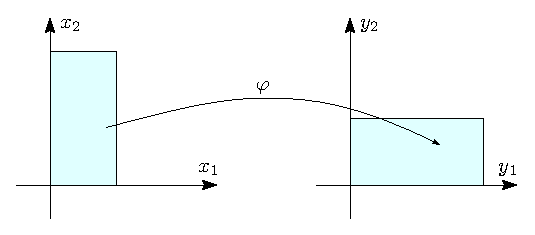
\includegraphics[width=0.5\textwidth]{MA4L6_1.eps}
		\caption{Частный случай функции перестановок для $n = 2$.}
		\label{6_1}
	\end{figure} 
	Тогда ФЗП будет иметь следующий вид:
	$$
		\ddint{\varphi(E)}{}f(y)dy = \ddint{E}{}f(\varphi(x))dx	
	$$
	Разместим $\ovl{E}$ внутрь некоторого замкнутого бруска $\MI$: $\ovl{E} \subset \Circ{\MI}$, $\varphi(\MI) = \MJ$ - замкнутый брус, поскольку мы просто меняем отрезки местами, как для примера с $n = 2$. Функция $f$ определена на $\varphi(E)$, доопределим $f$ на $\MR^n$, тогда по определению:
	$$
		\ddint{\varphi(E)}{}f(y)dy = \ddint{\MJ = \varphi(\MI)}{}f(y)\chi_{\varphi(E)}(y)dy, \quad \ddint{E}{}f(\varphi(x))dx = \ddint{\MI}{}f(\varphi(x))\chi_{E}(x)dx
	$$
	Заметим, что: $\chi_{\varphi(E)}(\varphi(x)) = \chi_{E}(x)$, обозначим $g(y) = f(y)\chi_{\varphi(E)}(y)$ тогда:
	$$
		f(\varphi(x))\chi_{E}(x) =f(\varphi(x))\chi_{\varphi(E)}(\varphi(x)) = g(\varphi(x)) 
	$$
	Следовательно, достаточно проверить равенство для бруса $\MI$:
	$$
		\ddint{\MJ = \varphi(\MI)}{}f(y)dy = \ddint{\MI}{}f(\varphi(x))dx 
	$$
	Возьмём $\MTB = \{\MI_m\}$ - разбиение бруса $\MI$, тогда $\MTB_\varphi = \{\varphi(\MI_m)\}$ - разбиение $\varphi(\MI)$ и $\lambda(\MTB) = \lambda(\MTB_\varphi)$.
	\begin{figure}[H]
		\centering
		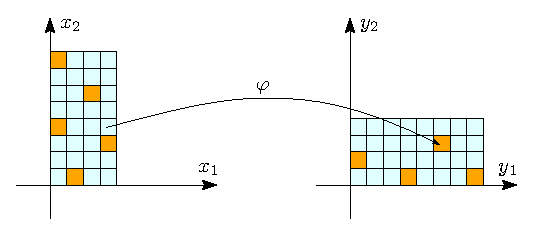
\includegraphics[width=0.5\textwidth]{MA4L6_2.eps}
		\caption{Частный случай отображения разбиения для $n = 2$.}
		\label{6_2}
	\end{figure} 
	Выберем точку $\xi_m \in \MI_m \Rightarrow \varphi(\xi_m) \in \varphi(\MI_m)$, запишем Риманову сумму:
	$$
		\ddsum{m}{}f(\varphi(\xi_m)){\cdot}|\varphi(\MI_m)| = \ddsum{m}{}f(\varphi(\xi_m)){\cdot}|\MI_m| 
	$$
	где равенство верно в силу того, что объем не меняется от перестановки мест множителей.
	$$
		\ddsum{m}{}f(\varphi(\xi_m)){\cdot}|\MI_m| \to \ddint{\MI}{}f(\varphi(x))dx, \, \ddsum{m}{}f(\varphi(\xi_m)){\cdot}|\varphi(\MI_m)| \to \ddint{\varphi(\MI)}{}f(y)dy \Rightarrow \ddint{\MI}{}f(\varphi(x))dx = \ddint{\varphi(\MI)}{}f(y)dy 
	$$
\end{proof}
\begin{proof}\hfill\\	
	\uline{Проверка формулы в частном случае $2)$}:	
	$$
		\varphi \colon \Omega_x = \MR^n \to \Omega_y =\MR^n, \, \varphi(x) = Ax + b, \, \det(A) \neq 0
	$$
	Множество $E$ это брус или получено из бруса аффинным невырожденным преобразованием (как $\varphi$). Это делаем для того, чтобы всегда знать, что сечения устроены хорошо (что это допустимые множества) и затем применить теорему Фубини. При таком определении сечения каждый раз будут выпуклым множеством и его одномерные сечения всегда будут промежутками. Пусть $f$ будет непрерывна на $\MR^n$. Проверим равенство:
	$$
		\ddint{\varphi(E)}{}f(y)dy = \ddint{E}{}f(\varphi(x)){\cdot}|\det{(A)}|dx
	$$
	Для случая $n = 2$ и нулевом $b$, мы получим:
	$$
		\varphi(x_1,x_2) = 
		\begin{pmatrix}
			a_{11} & a_{12}\\
			a_{21} & a_{22}
		\end{pmatrix}
		\begin{pmatrix}
			x_1 \\
			x_2
		\end{pmatrix}
	$$
	\begin{figure}[H]
		\centering
		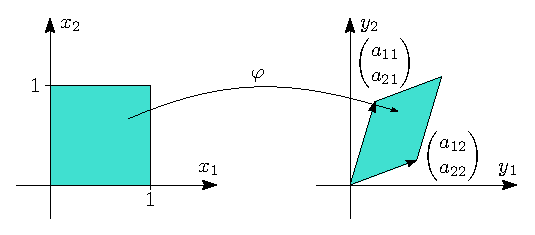
\includegraphics[width=0.5\textwidth]{MA4L6_3.eps}
		\caption{Частный случай преобразования для $n = 2$ и нулевом $b$.}
		\label{6_3}
	\end{figure}
	Если взять $f = 1$, то равенство означает: $|\varphi(E)| = |\det{(A)}|{\cdot}|E|$. Объем параллелограмма это определитель соответствующей матрицы (ориентированный, а неориентированный - с модулем). Далее, любая сложная фигура составляется из кубиков. И если теперь возьмем их образ, то получится, что образ этой фигуры составляется из параллелограммов. Площадь образа это площадь кубика, умноженного на константу $\Rightarrow$ вся площадь фигуры должна умножаться на эту константу. 
	\begin{figure}[H]
		\centering
		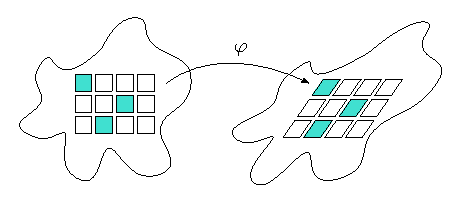
\includegraphics[width=0.5\textwidth]{MA4L6_4.eps}
		\caption{Общий подход к ФЗП.}
		\label{6_4}
	\end{figure}
	Переход к общей формуле замены объясняется так: мы знаем, что любой интеграл можно свести к сумме интегралов по маленьким кубикам $\Rightarrow$ для малого кубика, любое гладкое отображение мало отличается от своей аффинной части:
	$$
		\varphi(x) \approx \varphi(x_0) + \varphi'(x_0)(x - x_0)
	$$
	Для таких мы поняли, что формула верна $\Rightarrow$ для маленьких кубов надо умножать на модуль определителя $|\varphi'|$ в точке $x_0$, а после того, как мы перейдем на всё множество $E$ окажутся в разных точках разные $\varphi'(x_0) \Rightarrow$ под интегралом возник модуль определителя матрицы якоби.
	
	\begin{lemma}
		Всякое отображение: $\varphi(x) = Ax + b$ является композицией конечного набора отображений следующего вида:\hfill
		\begin{enumerate}[label=(\arabic*)]
			\item Переставление координат (смотри случай $1)$);
			\item $y_1 = x_1, \dotsc , y_{n-1} = x_{n-1}, y_n = x_n + c$, где $c$ - какое-то число;
			\item $y_1 = x_1, \dotsc , y_{n-1} = x_{n-1}, y_n = c{\cdot}x_n$, где $c$ - какое-то число;
			\item $y_1 = x_1, \dotsc , y_{n-1} = x_{n-1}, y_n = x_n + x_{n-1}$;
		\end{enumerate}
		То есть $\varphi = \varphi_1 \circ \varphi_2 \circ \dotsc \circ \varphi_m$, где каждое отображение является одного из этих видов.
	\end{lemma}
	\begin{proof}
		Это элементарные преобразования из метода Гаусса $\Rightarrow$ доказательство в алгебре.
	\end{proof}
	Как меняется объем при таких преобразованиях? При перестановке - не меняется. При $(2)$ мы сдвигаем проекцию $\Rightarrow$ по принципу Кавальери объем не меняется. При $(3)$ мы каждое сечение растягиваем в $c$ раз $\Rightarrow$ объем умножится в $|c|$ раз. При $(4)$ ничего не отличается от $(2)$, сдвигаем каждый раз на разные значения, сечение длин не меняется $\Rightarrow$ работает принцип Кавальери. Следовательно, мы знаем как меняется объем в каждом из этих случаев. Остальное докажем в следующий раз.
\end{proof}

\end{document}